\capitulo{4}{Técnicas y herramientas}
\section{Desarrollo ágil}
Durante la realización de esta segunda versión se ha mantenido la metodogía de desarrollo ágil siguiendo la línea de una evolución constante, permitiendo la obtención del feedback entre alumno y tutores de forma continua.
\subsection{Desarrollo iterativo}
El desarrollo consiste en la revisión cíclica sobre un mismo trabajo. En este caso se han realizado sprints de entre 7 y 14 días en los que se establecía una reunión en la plataforma Microsoft Teams al final del sprint mostrando los resultados y recibiendo una retroalimentación de los errores, posibles mejoras y características interesantes de implementar de cara al siguiente sprint. A partir del décimo sprint buscando una mejor comprensión del trabajo realizado se ha decidido incorporar el uso de milestones en GitHub.
\subsection{Desarrollo incremental}
El desarrollo incremental sigue la dinámica del desarrollo iterativo buscando la continua mejora gracias al feedback obtenido. Con este procedimiento se han ido realizando varias release a lo largo del trabajo. Una release es una nueva versión del sistema que se está desarrollando \cite{releasedefinition}.
\subsection{Control de versiones}
El control de versiones es un sistema que se utiliza para gestionar y controlar los cambios realizados en los archivos y documentos de un proyecto o sistema de software a lo largo del tiempo. Permite realizar un seguimiento de las modificaciones, controlar quién ha realizado cada cambio, revertir a versiones anteriores y colaborar de manera efectiva en el desarrollo de software.

El control de versiones es especialmente importante en el desarrollo de software, donde múltiples personas trabajan en el mismo proyecto y realizan cambios en los archivos de código fuente. Con un sistema de control de versiones, los desarrolladores pueden guardar y compartir las versiones de su código, fusionar los cambios realizados por diferentes personas y resolver conflictos que puedan surgir \cite{ZOLKIFLI2018408}.
\subsection{GitHub}
GitHub es una plataforma web de alojamiento y colaboración para proyectos de desarrollo de software que utiliza un sistema de control de versiones distribuido llamado Git. En este proyecto, GitHub ha sido utilizado como plataforma de alojamiento para almacenar y compartir el código fuente.

Una de las funcionalidades clave de GitHub es la capacidad de realizar \textit{push} de cambios a un repositorio. El \textit{push} es el acto de enviar los cambios locales a un repositorio remoto en GitHub. Esto permite a los desarrolladores compartir su código y colaborar con otros miembros del equipo de desarrollo \cite{10.1145/2675133.2675284}.
\subsection{Extensión de Visual Studio Code - Git Graph}
Git Graph es una extensión del editor de texto Visual Studio Code que proporciona una interfaz gráfica interactiva para visualizar y navegar por la historia de un repositorio de Git. Permite a los desarrolladores ver de manera intuitiva el historial de cambios, las ramas, las fusiones y las etiquetas de un proyecto Git.

Esta extensión muestra un gráfico visual en forma de árbol que representa la estructura del historial de commits del repositorio. Cada commit se muestra como un nodo en el gráfico y las líneas conectan los nodos para mostrar la relación entre ellos. Además, Git Graph proporciona información adicional sobre cada commit, como el autor, el mensaje de commit y la fecha, como se puede ver en la figura \ref{img:gitgraph}. 
\begin{figure}
  \centering
  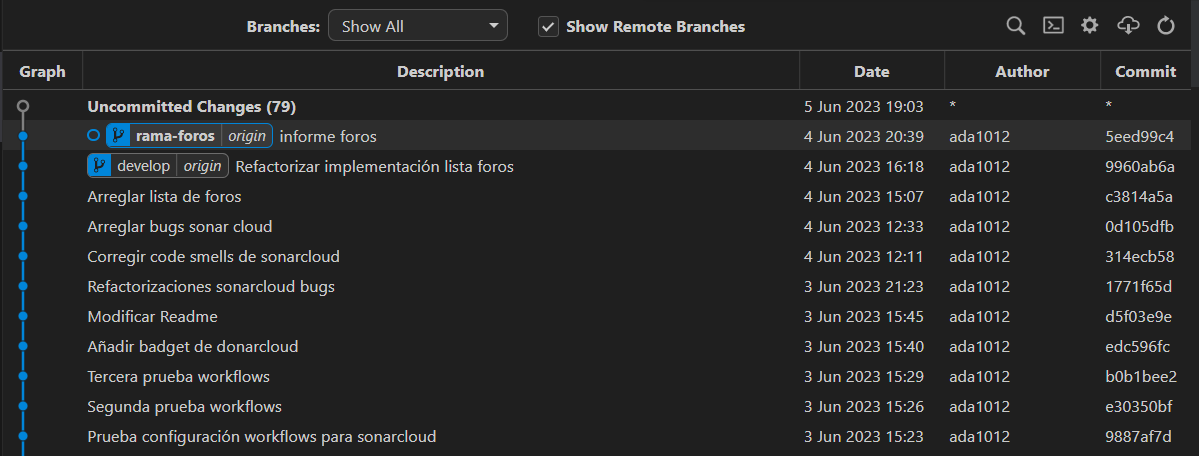
\includegraphics[width=1\textwidth]{GitGraph.png}
  \caption{Extensión de Visual Studio Code - Git Graph}
  \label{img:gitgraph}
\end{figure}
\subsection{Postman}
Es una aplicación que facilita el proceso de desarrollo, prueba y documentación de API (Interfaces de Programación de Aplicaciones). Proporciona una interfaz intuitiva y amigable que permite a los desarrolladores realizar solicitudes HTTP a servidores web y recibir respuestas en tiempo real. Con Postman, los usuarios pueden enviar diferentes tipos de solicitudes, como GET, POST, PUT y DELETE, así como configurar encabezados, parámetros y cuerpos de solicitud personalizados \cite{Christudas2019}.
\subsection{Publicaciones frecuentes}
Una publicación o release consiste en desplegar una aplicación funcional que permite la interacción de los usuarios con dicho producto. Durante el desarrollo del proyecto se han publicado 3 versiones.
\subsection{Refactorización}
La refactorización es el proceso de modificar el diseño interno de un código fuente sin cambiar su comportamiento externo. Se trata de mejorar la estructura y la calidad del código sin añadir nuevas funcionalidades o alterar su funcionalidad existente. El objetivo principal de la refactorización es hacer que el código sea más legible, mantenible y eficiente \cite{asse2015}. En este proyecto se ha implementado SonarCloud para detectar los fallos (\textit{bugs, code smells, vulnerabilities}) y posteriormente realizar dichas refactorizaciones .
\subsection{Uso de test unitarios}
Un test unitario es una técnica de pruebas en el desarrollo de software que tiene como objetivo verificar el correcto funcionamiento de una unidad de código, por lo general, una función, método o clase, de forma aislada e independiente del resto del sistema. En esta aplicación se ha utilizado JUnit para el desarrollo y posterior ejecución de los test \cite{8823472}.
\subsubsection{JUnit}
JUnit es un framework de pruebas unitarias en Java que proporciona un entorno para escribir, organizar y ejecutar pruebas de manera automatizada. Es ampliamente utilizado en el desarrollo de software para garantizar la calidad y funcionalidad de los componentes individuales del código \cite{8823472}.
\subsection{Construcción automática}
La construcción automática se refiere al proceso de utilizar herramientas especializadas, como Maven o Gradle, para automatizar tareas como la compilación del código fuente, la ejecución de pruebas y la generación de archivos de distribución del software. Estas herramientas permiten simplificar y agilizar el proceso de construcción del software, garantizando la consistencia y facilitando su integración en los flujos de trabajo de desarrollo.
\subsubsection{Maven}
Maven es una herramienta de gestión de proyectos de software ampliamente utilizada en el ecosistema de desarrollo de Java. Proporciona un enfoque estructurado y basado en convenciones para la construcción, gestión de dependencias y generación de proyectos. Maven simplifica la configuración y automatiza tareas comunes, como la compilación, la ejecución de pruebas, la generación de informes y la creación de distribuciones del software \cite{packt2014}.
\subsection{Integración continua}
La integración continua es una práctica de desarrollo de software en la que los cambios de código se integran y se prueban automáticamente de forma regular. Consiste en utilizar herramientas y sistemas de automatización para compilar, probar y validar el código constantemente. Esto permite detectar y solucionar errores de manera temprana, facilitando la entrega de software de calidad de forma rápida y frecuente. 
El proyecto contiene un archivo \texttt{yml} que especifica las acciones a seguir para la construcción automática del proyecto y el análisis de calidad de SonarCloud tras cada \textit{push} a la rama \textit{develop} del repositorio.
\subsection{Despliegue continuo}
El despliegue continuo es una práctica de desarrollo de software que automatiza el proceso de lanzamiento de nuevas versiones o actualizaciones de una aplicación, permitiendo entregar cambios de forma rápida y frecuente a través de integración, pruebas y despliegue automatizados. En este caso se ha empleado la herramienta Heroku: \texttt{\url{https://elearningqaquizandforums-bfe6b3c5090f.herokuapp.com/}}
\subsection{Heroku}
Heroku es una plataforma en la nube que permite el despliegue y alojamiento de aplicaciones web de manera sencilla, ofreciendo escalabilidad y administración simplificada.
\subsection{Herramienta de calidad de código: SonarCloud}
SonarCloud es una plataforma en la nube que ofrece servicios de análisis estático de código para evaluar la calidad del software. Proporciona un conjunto de herramientas y métricas que permiten identificar problemas de código, vulnerabilidades, duplicaciones y otras deficiencias en el código fuente. SonarCloud realiza un análisis exhaustivo y genera informes detallados sobre la calidad y la salud general del proyecto. Ayuda a los equipos de desarrollo a mejorar la mantenibilidad, la eficiencia y la seguridad del software mediante la identificación temprana de posibles problemas y la adopción de buenas prácticas de programación.
En este proyecto se integra con los \textit{actions} de GitHub para analizar el proyecto a la hora de realizar un push en la rama develop.
Se puede ver la evolución de la calidad del código en \url{https://sonarcloud.io/project/activity?category=QUALITY_GATE&id=ada1012_eLearningQA}.

\section{Herramientas de desarrollo}
\subsection{Entorno de desarrollo integrado: Eclipse y Visual Studio Code}
Por motivos personales en este trabajo se han utilizado dos entornos de desarrollo, Eclipse y Visual Studio Code. Esta decisión se ha tomado por la comodidad de configuración de archivos de Eclipse y la interfaz amigable de Visual Studio Code. Este último permite instalar varias extensiones como Git Graph o GitHub Copilot que hacen la programación mucho más amena.
\subsection{Extensión de Visual Studio Code - GitHub Copilot}
GitHub Copilot es una herramienta desarrollada por GitHub y OpenAI que utiliza inteligencia artificial (IA) para proporcionar sugerencias y autocompletar código mientras se escribe en diferentes lenguajes de programación. Funciona como una extensión para el editor de código y aprovecha los modelos de lenguaje generativos de OpenAI, como GPT-3, para ofrecer recomendaciones de código en tiempo real.
Esto permite obtener recomendaciones de código sin necesidad de acudir al navegador.
\subsection{Framework CSS: Bootstrap}
Bootstrap es un framework CSS de código abierto ampliamente utilizado en el desarrollo web. Proporciona una colección de estilos predefinidos, componentes y utilidades que permiten crear interfaces web responsivas y atractivas de manera rápida y sencilla. Bootstrap facilita la creación de diseños flexibles y adaptables a diferentes dispositivos, optimizando la experiencia del usuario en diversos tamaños de pantalla. Además, ofrece funcionalidades como tipografía, estilos de botones, formularios, navegación y mucho más, lo que agiliza el desarrollo de sitios web con un aspecto profesional \cite{bootstrap}.
\subsection{Librería de generación de gráficos: Plotly}
Plotly es una librería de generación de gráficos interactivos y visualizaciones de datos en varios lenguajes de programación, como Python, R y JavaScript. Proporciona una amplia gama de tipos de gráficos, incluyendo gráficos de dispersión, líneas, barras, áreas, mapas y más. Plotly permite personalizar los gráficos con facilidad, añadir interactividad como zoom y desplazamiento, y compartir los gráficos generados en la web. Además, ofrece capacidades de colaboración y una API que facilita la integración con otras herramientas y aplicaciones \cite{10.1111/rssa.12692}.

\section{Herramientas de documentación}
\subsection{Redacción de memoria y anexos: Overleaf}
Overleaf es una herramienta en línea de colaboración y edición de documentos LaTeX. Permite a los usuarios crear, editar y compilar documentos LaTeX en un entorno en la nube, sin necesidad de instalar software adicional. Overleaf es especialmente popular entre la comunidad académica y científica, ya que facilita la colaboración en tiempo real y simplifica el proceso de escritura de documentos técnicos y científicos \cite{overleaf}.
\subsection{Generación de diagramas UML: Dia}
Dia es una aplicación de software de código abierto que se utiliza para la creación y edición de diagramas UML (Unified Modeling Language, o Lenguaje de Modelado Unificado). Permite a los usuarios diseñar diagramas UML, como diagramas de clases, diagramas de casos de uso, diagramas de secuencia, diagramas de actividad y más.

\section{Patrón de diseño: Fachada}
El patrón de diseño Fachada proporciona una interfaz simplificada y unificada para acceder a subsistemas o clases complejas, ocultando su complejidad y facilitando la interacción con el sistema. En otras palabras, ofrece una interfaz que centraliza el control de la aplicación y maneja el trabajo de cada subsistema.
Este patrón de diseño aumenta la portabilidad de la aplicación ya que permite trasladar en pocos pasos la aplicación web a una aplicación de escritorio o a una aplicación móvil minimizando los cambios requeridos \cite{mendia2019}.

 \section{Herramientas para acceder a la información}
En este apartado se va a explicar cómo se ha accedido a la información de los cursos de Moodle y las opciones que se han barajado durante las reuniones con los tutores.
\subsection{Opción elegida - Web services}
Web services son conjuntos de protocolos y estándares que permiten la comunicación y el intercambio de datos entre diferentes aplicaciones o sistemas a través de la web. Utilizando HTTP como protocolo de transporte, los web services permiten que las aplicaciones se comuniquen y compartan información de manera interoperable e independiente de la plataforma.

Los web services de Moodle, un sistema de gestión de aprendizaje en línea, proporcionan interfaces de programación (API) que permiten la integración de Moodle con otras aplicaciones. Estos web services permiten realizar operaciones como la autenticación de usuarios, el acceso a recursos y actividades del curso y la obtención de datos relacionados con los usuarios, cursos y calificaciones.
\subsection{Opción planteada - Web scraping}
Web scraping es una técnica automatizada que consiste en extraer y recopilar datos de manera estructurada de sitios web. Esta técnica implica el uso de software o scripts para acceder a las páginas web, analizar su contenido y extraer la información deseada, como texto, imágenes, enlaces u otros datos relevantes.
Al final no se eligió esta opción ya que la mayoría de información que requería la aplicación ya la ofrecía Moodle a través de sus web services.

\section{Framework de desarrollo web}
El framework elegido para el desarrollo del proyecto ha sido heredado de la versión anterior \cite{previotfg}.
\subsection{Spring}
Spring es un framework de desarrollo de aplicaciones empresariales para la plataforma Java. Proporciona una infraestructura completa y coherente que facilita la creación de aplicaciones escalables y de alta calidad. Spring se basa en los principios de inversión de control (IoC) y la inyección de dependencias (DI), lo que permite una mayor modularidad, flexibilidad y facilita las pruebas unitarias. Además, Spring ofrece una amplia gama de módulos y funcionalidades que abarcan desde la creación de servicios web hasta la integración con bases de datos y la seguridad.